\section{TCP/IP 소켓통신을 이용한 데이터 송/수신}
Socket programming (TCP/IP)을 통해 src.jpg 파일을 4096 Bytes 단위로 나누어 송/수신했다.

\subsection{Code}
\vspace{-4mm}
\begin{listing}[h!]
\inputminted[framerule = 1pt,framesep = 2mm , frame = lines, fontsize=\footnotesize]{python}{./code/week09/02/webserver.py}
\caption{\footnotesize Experiment 2, webserver.py}
\end{listing}
\clearpage

\vspace{-4mm}
\begin{listing}[h!]
\inputminted[framerule = 1pt,framesep = 2mm , frame = lines, fontsize=\footnotesize]{python}{./code/week09/02/client.py}
\caption{\footnotesize Experiment 2, client.ipynb}
\end{listing}

\subsection{Process Analysis}
\begin{enumerate}
    \item TCP/IP Server/Client socket 생성(socket) 및 Server의 IP 주소와 Port 번호 설정(bind)
    \item Server가 Client로부터 연결 요청이 있는지 수신 대기(listen)
    \item Client가 IP 주소와 Port 번호로 식별되는 Server에게 연결 요청(connect)
    \item Server가 Client의 연결 요청을 수락(accept)
    \item Client가 Server에게 src.jpg 파일을 요청하는 메세지 송신(send/recv)
    \item Server는 src.jpg 파일을 읽고 4096 Bytes 단위로 나누어 Client에게 모든 데이터를 보낼 때까지 송신 반복(send/recv)
    \item Client는 받은 파일을 새로운 src.jpg에 write
    \item Client socket close으로 TCP connection 종료
\end{enumerate}

\subsection{Experiment Result}
Client가 Server에게 src.jpg 파일을 요청했고, Server는 src.jpg를 4096 Bytes 단위로 38개의 packet으로 나누어 송신했다. \\
\vspace{-4mm}
\begin{figure}[!h]\centering 
	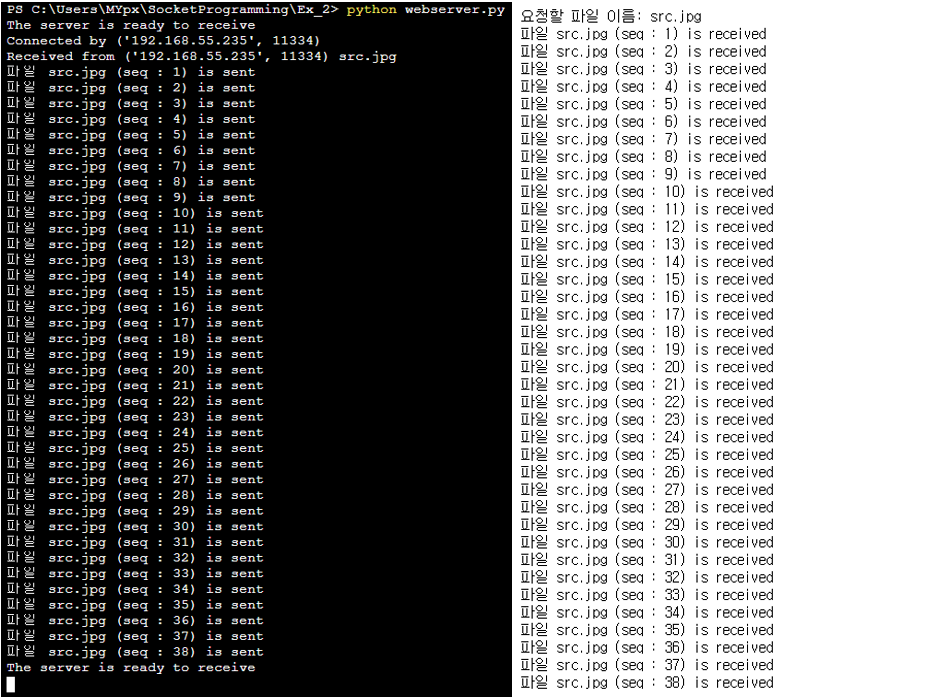
\includegraphics[width=.99\textwidth]{image/week09/2-1.png}
	\caption{\footnotesize
	Server Terminal and Client on Jupiter Notebook}
	\vspace{-10pt}
\end{figure}

Client 폴더 내에 src.jpg가 생성되었다. \\
\vspace{-4mm}
\begin{figure}[!h]\centering 
	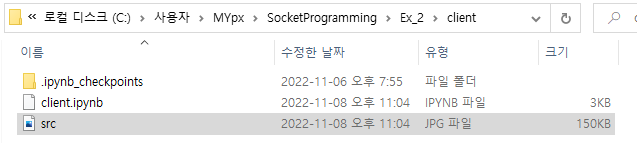
\includegraphics[width=.99\textwidth]{image/week09/2-2.png}
	\caption{\footnotesize
	src.jpg in client directory}
	\vspace{-10pt}
\end{figure}
\vspace{-4mm}
\begin{figure}[!h]\centering 
	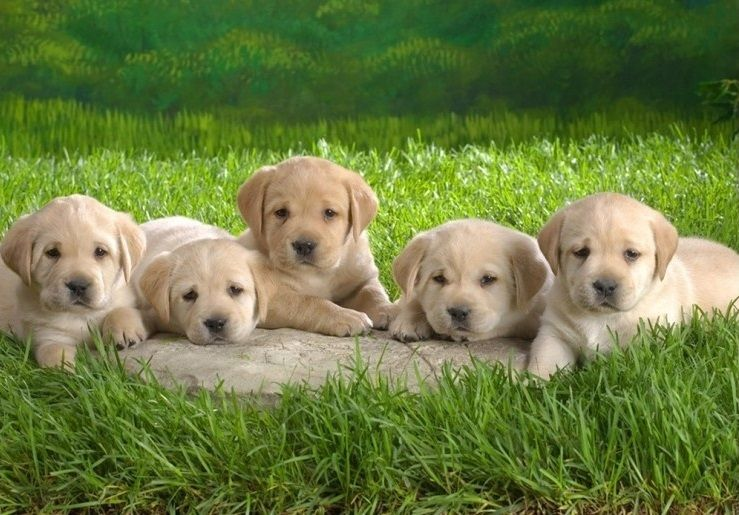
\includegraphics[width=.99\textwidth]{image/week09/2-3.png}
	\caption{\footnotesize
	src.jpg received by client}
	\vspace{-10pt}
\end{figure}

\clearpage